\section{Results}

\subsection{Main empirical takeaway}

The frozen discovery-ablation package does not support a claim that one model
dominates every stratum. Instead, it supports a more conservative and more
useful conclusion: model choice is age-dependent and objective-dependent.
Observation-aware constrained discovery is most compelling for the pediatric
\texttt{0-4 yr} series, while adult strata often favor simple forecasting
baselines or hand-specified epidemic models.

\subsection{No single global winner}

Table~\ref{tab:frozen-recommendations} summarizes the paper-ready
recommendation table derived from
\texttt{artifacts\_discovery\_ablation/paper\_recommendation\_table.csv}. The
table reports both held-out test and rolling-origin winners because these
objectives do not always agree.

\begin{figure}[H]
\centering
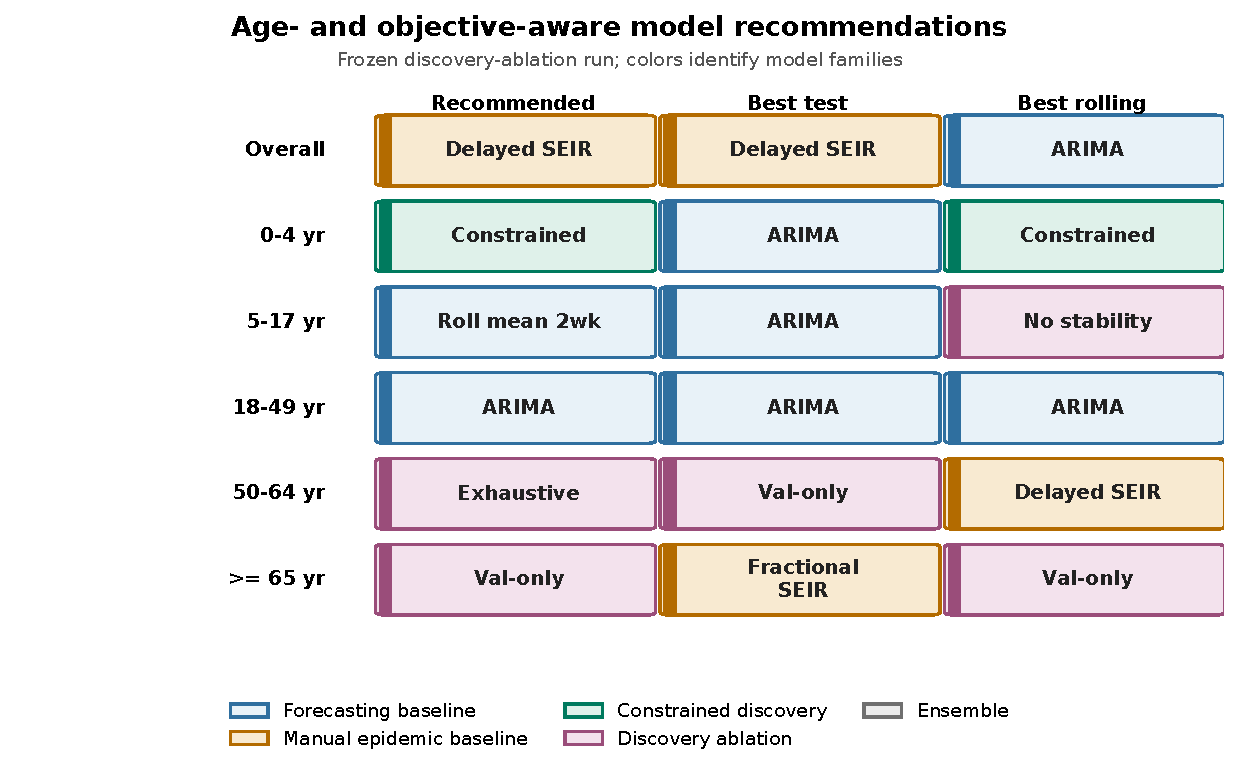
\includegraphics[width=\textwidth]{figures/fig1_recommendation_map.pdf}
\caption{Age- and objective-aware model recommendations from the frozen
discovery-ablation run. Different age strata favor different model families
and different evaluation objectives. The figure therefore supports
objective-aware recommendation rather than a single global winner claim.}
\label{fig:recommendation-map}
\end{figure}

\begin{table}[H]
\centering
\small
\caption{Frozen recommendation summary from the discovery-ablation run. The
recommended model is the benchmark policy output, not a claim of universal
dominance.}
\label{tab:frozen-recommendations}
\begin{tabularx}{\textwidth}{>{\raggedright\arraybackslash}p{1.35cm}
>{\raggedright\arraybackslash}p{3.1cm}
>{\raggedright\arraybackslash}p{2.25cm}
>{\raggedright\arraybackslash}p{2.8cm}
>{\raggedright\arraybackslash}p{2.8cm}
X}
\toprule
Series & Recommended model & Decision type & Best test model & Best rolling model & Selected discovery structure \\
\midrule
Overall & \texttt{delayed\_observation\_seir} & test preferred &
\texttt{delayed\_observation\_seir} & \texttt{arima\_auto\_small} & -- \\
\texttt{0-4 yr} & \texttt{constrained\_structure\_discovery} &
stability preferred & \texttt{arima\_auto\_small} &
\texttt{constrained\_structure\_discovery} &
\texttt{SEIRS}, \texttt{delayed\_I}, delay 1 \\
\texttt{5-17 yr} & \texttt{rolling\_mean\_2wk} & balanced tradeoff &
\texttt{arima\_auto\_small} & \texttt{no\_stability\_discovery} & -- \\
\texttt{18-49 yr} & \texttt{arima\_auto\_small} & consensus &
\texttt{arima\_auto\_small} & \texttt{arima\_auto\_small} & -- \\
\texttt{50-64 yr} & \texttt{exhaustive\_structure\_discovery} &
balanced tradeoff & \texttt{validation\_only\_structure\_selection} &
\texttt{delayed\_observation\_seir} & \texttt{SIR}, \texttt{I}, delay 0 \\
\texttt{>= 65 yr} & \texttt{validation\_only\_structure\_selection} &
stability preferred & \texttt{fractional\_seir} &
\texttt{validation\_only\_structure\_selection} &
\texttt{SEIRS}, \texttt{I}, delay 0 \\
\bottomrule
\end{tabularx}
\end{table}

As an unfiltered descriptive average across the six frozen series,
\texttt{constrained\_structure\_discovery} has the lowest mean test MAE
(\num{0.0561}), followed closely by
\texttt{validation\_only\_structure\_selection} (\num{0.0562}). This aggregate
is not used as a global-win claim because some rows are numerically flagged
and because series-level winners differ. For example, the \texttt{Overall}
held-out split favors \texttt{delayed\_observation\_seir}, while
\texttt{18-49 yr} favors \texttt{arima\_auto\_small} under both test and
rolling-origin metrics.

\subsection{Pediatric 0-4 yr is the strongest positive discovery finding}

The clearest positive discovery result is the pediatric \texttt{0-4 yr}
series. The benchmark recommends
\texttt{constrained\_structure\_discovery} as the stability-preferred model,
and the rolling-origin winner is also
\texttt{constrained\_structure\_discovery}. The selected structure is
\texttt{SEIRS} with a delayed infectious observation map
\texttt{delayed\_I} and delay 1.

This is the strongest setting for the observation-aware discovery story
because the selected delayed-observation structure is not merely a more complex
variant of a manual SEIR baseline: it is selected by the constrained grammar
and remains favorable under rolling-origin evaluation. The paired
rolling-origin comparison further supports this interpretation. Against the
observation-fixed ablation, constrained discovery reduces rolling absolute
error by \num{0.0564} on average for \texttt{0-4 yr}, with a bootstrap
95\% confidence interval from \num{0.0173} to \num{0.1082}.

\subsection{Observation-search ablation evidence}

Figure~\ref{fig:observation-search-impact} and
Table~\ref{tab:observation-search-impact} compare
\texttt{constrained\_structure\_discovery} with
\texttt{no\_observation\_search\_discovery}. Positive deltas mean the
observation-fixed ablation has higher error, so constrained discovery is
better. The full table is
\texttt{artifacts\_discovery\_ablation/observation\_search\_impact\_table.csv}.

\begin{figure}[H]
\centering
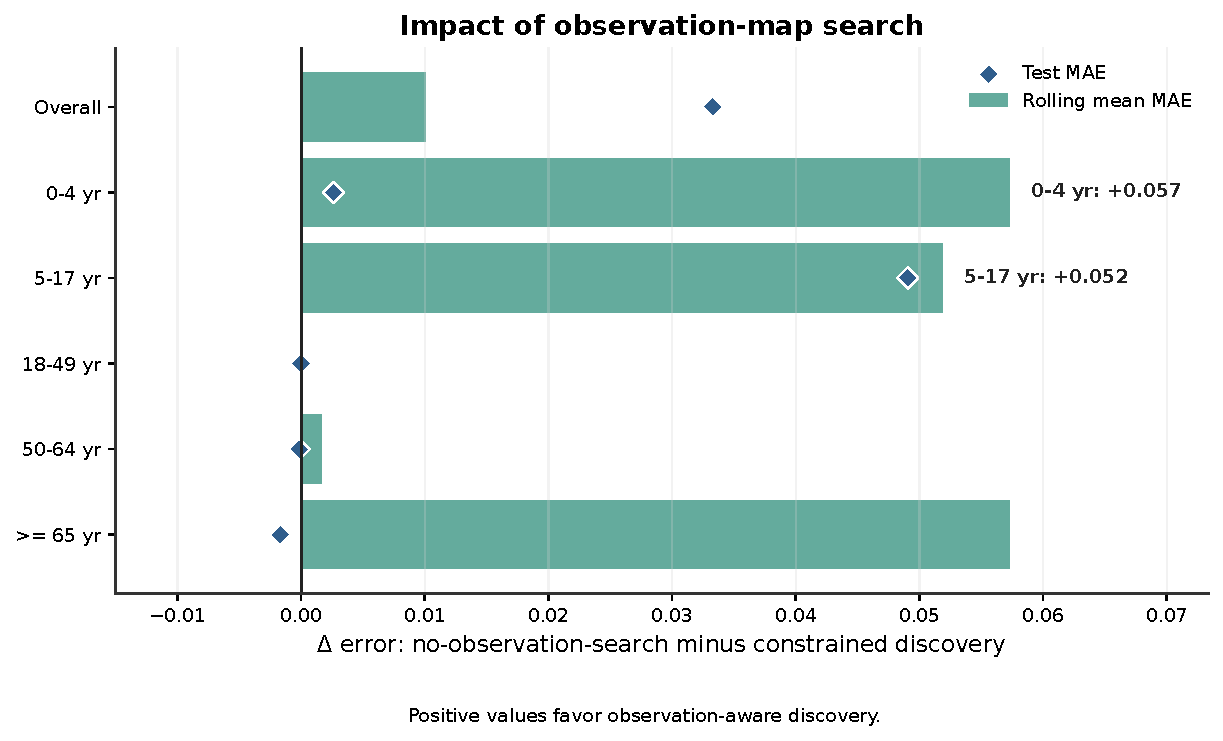
\includegraphics[width=0.98\textwidth]{figures/fig2_observation_search_impact.pdf}
\caption{Impact of observation-map search. Positive values mean that the
observation-fixed ablation has higher error than constrained discovery. The
clearest positive signal is in the pediatric strata, especially
\texttt{0-4 yr}, where observation-aware constrained discovery selects a
delayed infectious observation map and improves rolling-origin stability.}
\label{fig:observation-search-impact}
\end{figure}

\begin{table}[H]
\centering
\small
\caption{Impact of disabling observation-map search. Positive deltas favor
constrained discovery. The \texttt{>= 65 yr} discovery rows include numerical
failure flags and should be interpreted descriptively rather than as positive
evidence.}
\label{tab:observation-search-impact}
\begin{tabular}{lcccc}
\toprule
Series & $\Delta$ test MAE & $\Delta$ rolling MAE & Constrained obs. & Fixed obs. \\
\midrule
Overall & \num{0.0333} & \num{0.0100} & \texttt{I} & \texttt{I} \\
\texttt{0-4 yr} & \num{0.0026} & \num{0.0573} & \texttt{delayed\_I} & \texttt{I} \\
\texttt{5-17 yr} & \num{0.0491} & \num{0.0519} & \texttt{delayed\_I} & \texttt{I} \\
\texttt{18-49 yr} & \num{-0.0000} & \num{-0.0000} & \texttt{I} & \texttt{I} \\
\texttt{50-64 yr} & \num{-0.0002} & \num{0.0017} & \texttt{I} & \texttt{I} \\
\texttt{>= 65 yr} & \num{-0.0017} & \num{0.0573} & \texttt{I} & \texttt{I} \\
\bottomrule
\end{tabular}
\end{table}

The observation-search effect is therefore not uniform. In several adult
series, both constrained and fixed-observation searches select \texttt{I},
producing little or no difference. In pediatric strata, especially
\texttt{0-4 yr}, allowing the search to choose delayed infectious observation
materially improves rolling-origin stability.

\subsection{Adult strata remain competitive for simple and manual baselines}

The adult groups are important negative evidence against overclaiming. The
\texttt{18-49 yr} series is best served by \texttt{arima\_auto\_small} in both
the held-out test split and rolling-origin evaluation. In paired rolling-origin
comparison, \texttt{arima\_auto\_small} has lower rolling absolute error than
constrained discovery for \texttt{18-49 yr}, with mean difference
\num{-0.0487} and a 95\% interval from \num{-0.0641} to \num{-0.0323}. On the
\texttt{Overall} series, \texttt{arima\_auto\_small} is also stronger by
rolling-origin MAE, while \texttt{delayed\_observation\_seir} is the best
held-out test model.

These results are useful because they show that the benchmark is not tuned to
force a discovery win. The discovery machinery identifies useful structure in
selected strata, but it also exposes cases where simple forecasting or manual
epidemic baselines are sufficient.

\begin{figure}[H]
\centering
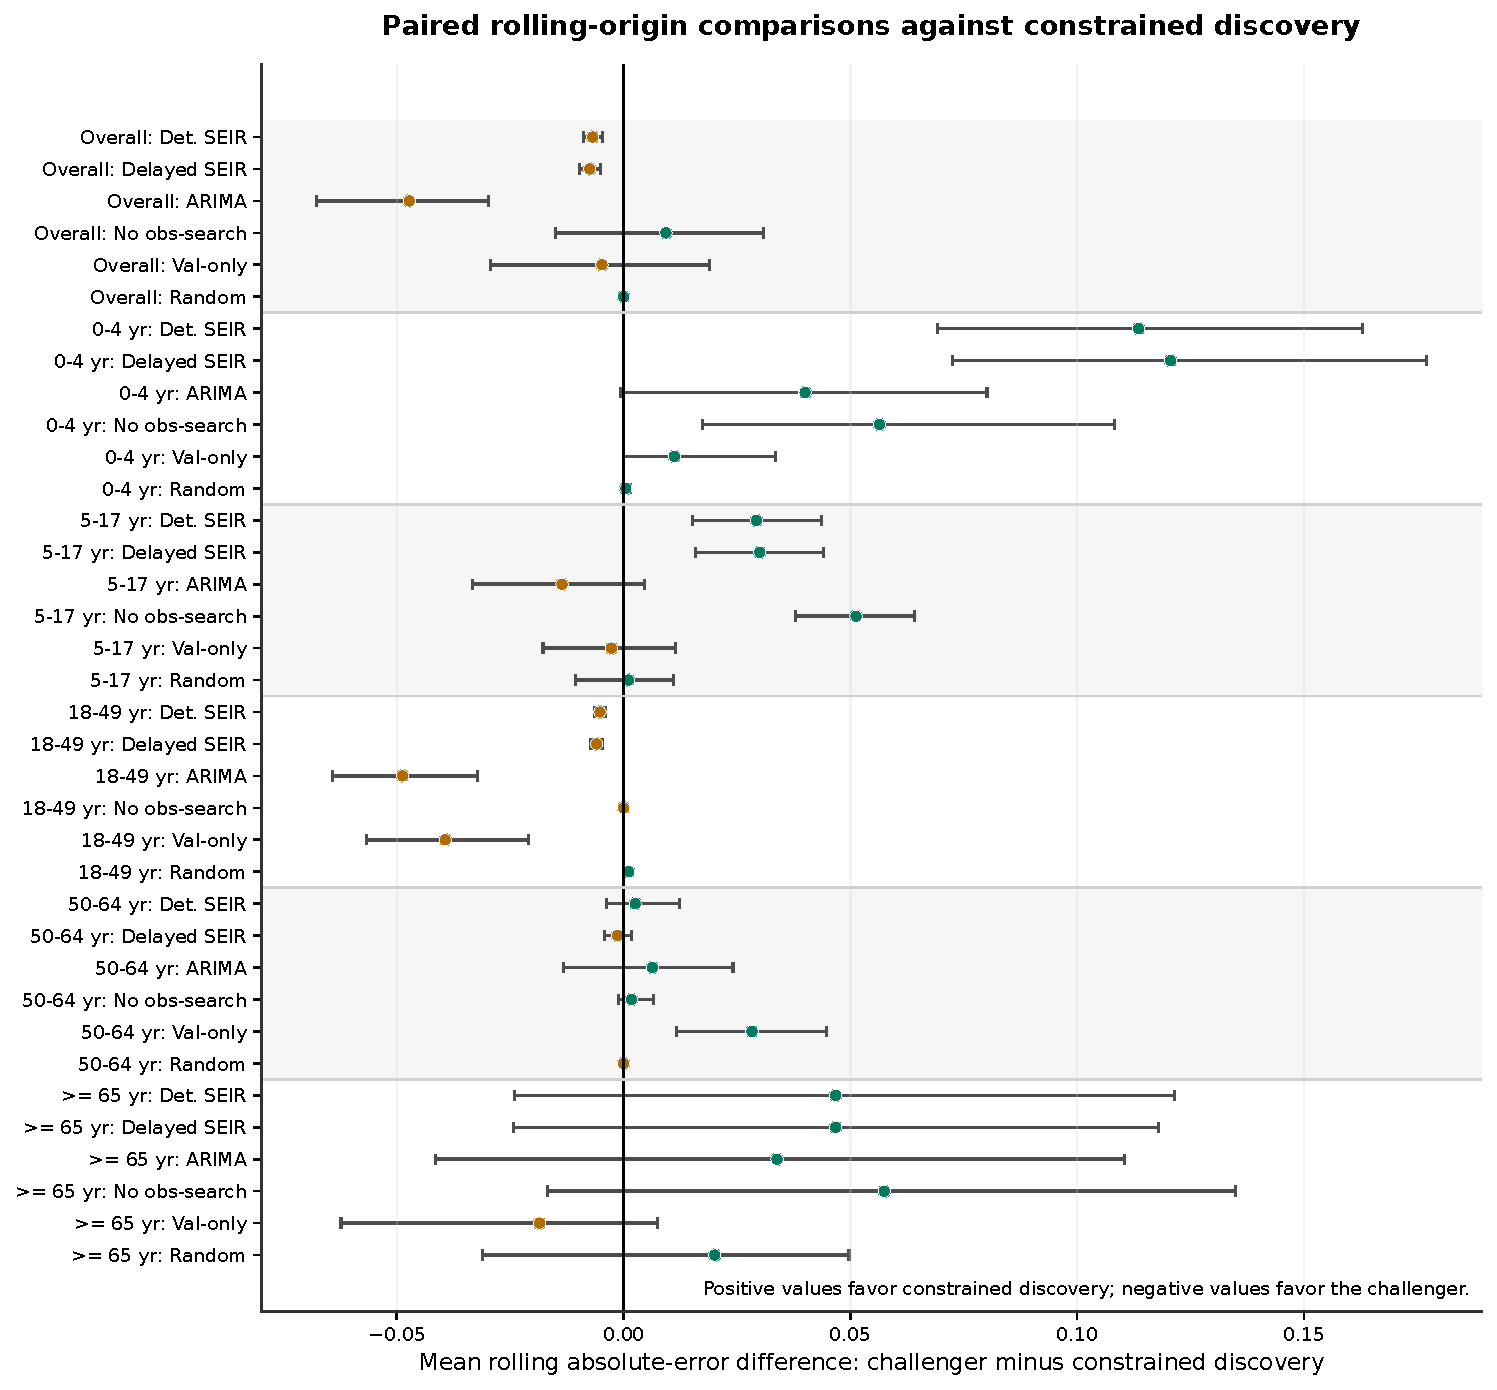
\includegraphics[width=\textwidth]{figures/fig4_paired_rolling_forest.pdf}
\caption{Post-hoc paired rolling-origin comparisons against constrained
discovery. Points show the mean rolling absolute-error difference
(\emph{challenger minus constrained discovery}) and intervals show bootstrap
95\% confidence intervals after aligning forecasts by series, horizon, and
target week. Positive values favor constrained discovery; negative values
favor the challenger. These comparisons summarize evidence after model
selection and are not used for model selection.}
\label{fig:paired-rolling-forest}
\end{figure}

\subsection{Objective-dependent recommendations}

Several series have different test and rolling winners. The \texttt{50-64 yr}
series has \texttt{validation\_only\_structure\_selection} as the best test
model, but \texttt{delayed\_observation\_seir} as the best rolling-origin
model. The \texttt{>= 65 yr} series has \texttt{fractional\_seir} as the best
test model and \texttt{validation\_only\_structure\_selection} as the best
rolling model. The \texttt{Overall} series similarly splits between
\texttt{delayed\_observation\_seir} on test MAE and
\texttt{arima\_auto\_small} on rolling-origin MAE.

The appropriate paper claim is therefore objective-aware and age-aware:
recommendations should state whether the priority is a fixed held-out split,
rolling-origin stability, or interpretability. The frozen artifacts support
this policy framing more strongly than a single leaderboard winner.

\subsection{Numerical failure audit}

The frozen summary retains numerical diagnostics for every model-series row.
There are 11 flagged rows among 108 model-series evaluations. The most common
flagged model is \texttt{hospitalized\_seihr}, with five flagged series. The
flagged rows are listed in
\texttt{artifacts\_discovery\_ablation/numerical\_failure\_summary.csv} and
summarized in \texttt{reports/numerical\_failure\_audit.md}.

Models flagged for numerical instability are retained for transparency but are
not used to support positive claims. This is particularly relevant for any
interpretation involving the flagged \texttt{>= 65 yr} constrained-discovery
row.
